\documentclass{acm_proc_article-sp}
\usepackage{booktabs}
\usepackage{url}
\usepackage{placeins}
\usepackage{listings}
\usepackage{multicol}
\usepackage{blindtext, subfig}
\usepackage{dblfloatfix} % fix for bottom-placement of figure

\lstset{breaklines=true}

\begin{document}

\title{Coevolution between iAnts and Obstacles\titlenote{The first project for CS 491 at The University of New Mexico}}

\numberofauthors{2}
\author{
\alignauthor
Troy M. Squillaci\\
       \affaddr{University of New Mexico}\\
       \affaddr{Department of Computer Science}\\
       \affaddr{Albuquerque, New Mexico}\\
       \email{zivia@unm.edu}
}

\maketitle
\begin{abstract}
This report presents results from investigating how autonomous robot ant swarms can forage for food in the presence of co-evolved obstacles. In particular, we discuss how coevolution, by a genetic algorithm, of ant behaviors and obstacle placements can directly influence the ants' ability to forage for food. We demonstrate how changing even a single behavior can affect the ants' ability to forage. Lastly, we examine challenges introduced by adding a variety of obstacles in the environment.

\textbf{0. Author Contributions} \\
Both authors contributed to the quality of this report and each section thereof. In particular, Troy Squillaci and Jake Nichol each wrote Python code to generate data used in figures and analysis. Troy wrote the genetic algorithm, code to generate most figures, and the core framework. Jake created the different specialized arenas for ant traps and the double bridge experimement. He also wrote Python scripts to generate data and figures for miscellaneous portions of the paper. Each author spent time improving the effectiveness of the genetic algorithm. Finally, this report was written by each author, jointly. 

\end{abstract}

\section{Introduction}
Our intention is to evolve efficient foraging strategies for a set of environments. We define an environment to be an arena with a centrally located nest and food tags distributed throughout, the means of distribution is described below. 

Environmental changes are constituted by altering food distribution. Three types of food distributions are used to diversify the environments:
\begin{itemize}
	\item Random Distribution - Food tags are uniformly distributed at random throughout the arena.

	\item Cluster Distribution - Food tags are split into square groups of equal size. The groups are uniformly distributed at random throughout the arena.

	\item Power Law Distribution - A mixture of both random distribution and cluster distribution. Clusters vary as follows: one 8x8 cluster, four 4x4 clusters, sixteen 2x2 clusters, and sixty-four 1x1 clusters (just one tag).
\end{itemize}

\begin{figure}[h]
\includegraphics[width=9cm]{images/FoodDistributions}
\caption{The three different food distributions used in our experiments. (a) illustrates a random distribution, (b) illustrates a clustered distribution, and (c) illustrates a power-law distribution.} \label{fig:foodDistributions}
\end{figure}

Later on, we add a specific set of obstacles to the arena. These obstacles form "bug traps," which are discussed in depth in Section \ref{sec:obstacles}.

Ant swarms are tasked with collecting as much food as possible within an environment. Foraging strategies are used in an attempt to collect as much food as possible. A foraging strategy is defined by a set of behaviors which are represented as central-place foraging algorithm (CPFA) parameters. CPFA parameters are described in the Keywords section of this paper. We calculate the fitness of a swarms' foraging strategy, within a given environment, by $\frac{the\ amount\ of\ food\ collected}{the\ amount\ of\ food\ available}$. 

The CPFA is an algorithm for autonomous swarm systems, which searches for and collects resources. A good description of the CPFA is given by Hecker\cite{hecker:CPFA}. See Figure \ref{fig:CPFA}.

\begin{figure*}[t]
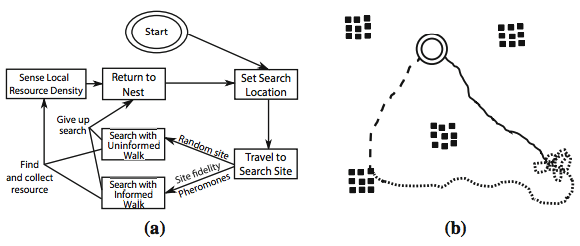
\includegraphics[width=18cm]{images/CPFA}
\caption{(a) State diagram describing the flow of behavior for individual robots during an experiment. (b) An example of a single cycle through this search behavior. The robot begins its search at a central nest site (double circle) and sets a search location. The robot then travels to the search site (solid line). Upon reaching the search location, the robot searches for resources (dotted line) until a resource (square) is found and collected. After sensing the local resource density, the robot returns to the nest (dashed line)\cite{hecker:CPFA}} \label{fig:CPFA}
\end{figure*}

A few important parameters, in the CPFA, include pheromone rate, pheromone decay rate, and site fidelity rate. Pheromones refer to invisible trails that the ants leave behind when they bring food back to the nest. Pheromone trails can be followed by any ant, thus, they act as a recruiting device to bring more ants to areas full of food. Pheromone rate is the frequency at which pheromones are laid. Pheromone decay rate is how quickly pheromones evaporate. This is important because pheromones may lead to areas that have already been exhausted of food. Site fidelity a memory mechanism which robots use to travel back to previously discovered food sites. Site fidelity rate is the frequency at which site fidelity is used.

In this paper we examine our experiments, the results, and their significance. In particular, we report on the following:

\begin{itemize}
	\item We show that altering a small subset of CPFA parameters - search radius, pheromones, and site fidelity - can have significant, yet predictable effects.
	\item How the significance of a CPFA parameter may depend on the current environment. We hypothesize that food distributions will effect pheromones and site fidelity the most, while obstacles will effect distance tolerance, angle tolerance, and search step size the most.
	\item The development of a genetic algorithm to specialize ant robot swarms for food foraging in a variety of environments.
	\item Optimal solutions may take different amounts of time to discover based on the environment. We believe that less structured environments, such as random distributions, will require less effort to develop such strategies.
	\item We make relative comparisons between the results of specialized swarms, for each environment.
\end{itemize}

\section{Results}
Below we discuss the results of our tests and analyze their meaning. An important note, pheromone rate and site fidelity rate are defined by the range always[0.0, 20.0]never. This means that when the value is larger, the strategy is used less. This is the definition in the ARGoS simulator and not of our choosing. Also all experiments involving the GA are run with a search radius of 0.23.

\begin{figure*}[ht]
\centering
\subfloat[][]{
   \includegraphics[width=6cm]{Plots/Part1/PheromoneRate10SiteFidelityRate10}
 }
\subfloat[][]{
   \includegraphics[width=6cm]{Plots/Part1/PheromoneRate0SiteFidelityRate20}
 }
\subfloat[][]{
   \includegraphics[width=6cm]{Plots/Part1/PheromoneRate20SiteFidelityRate0}
 }
\caption{(a) The average number of food tags collected over 10 simulations, using default parameters, pheromone and site fidelity used equally, and a search radius at 0, 0.23, and 1. (b) The average number of food tags collected over 10 simulations, using default parameters, using only pheromones, and a search radius at 0, 0.23, and 1. (c) The average number of food tags collected over 10 simulations, using default parameters, using only site fidelity, and a search radius at 0, 0.23, and 1.} \label{fig:part1}
\end{figure*}

\subsection{The Importance of Search Radius} \label{sec:part1}

In this section we analyze how the robots' search radius parameter affects their ability to find food. The search radius parameter is only used when an ant finds a food tag and performs a 360 degree search around itself to determine how much food is nearby. When site fidelity is used, the amount of food an ant sees will determine the likelihood of the ant returning to this area to search for the previously spotted food. When pheromones are used, the amount of food an ant sees will determine how much pheromone is laid on the way back to the nest.

We examine three different radii, 0.0, 0.23, and 1.0. These three were chosen because of the following: with a search radius of 0, the ants cannot see any tags around them; with a search radius of 0.23, the ants can only see tags directly next to them (a maximum of 8 - left, right, in front, behind, and the four diagonals); and with a search radius of 1, the ants can see entire meter away and all of the tags within.

With a search radius of one, an ant arriving at a cluster will see most of the cluster at once, knowing for sure that it is a good place to return to. This leads to the hypothesis that a larger search radius helps the swarm perform much better because they can better utilize their tools of site fidelity and pheromone trails to return to the better areas. However, this is not always true. 

In Figure \ref{fig:part1}(a), pheromone trails and site fidelity are used equally. This allows for the differences created by search radius to emerge more clearly. Look closely at which radii produce the best results in each distribution. 

When the ants are foraging in an environment with a random distribution of food, smaller search radii allow for the swarms to perform much better. This is because when the ants can only see nearby food tags, especially in the case of a zero search radius, they treat the search space as random. When an ant finds a tag in a large pile of tags, it is no more likely to return to that area than any other. 

This explains why the swarms do not perform worse in a random environment, but the swarms actually perform better. Because the ants treat all collected tags the same, they spend most of their time searching, rather than returning to previously discovered food piles. In a clustered distribution, the food is compact and there are large areas of the arena that are devoid of food tags. In a random distribution, food is uniformly spread throughout the arena. This means that when an ant starts a new search, it is likely to find a tag quickly. In power-law distributions, most food tags are in clusters, so we see that larger search radii perform better.

In Figure \ref{fig:part1}(b), we look at the same circumstances as in Figure \ref{fig:part1}(a), but site fidelity is never used and pheromones are always used. In this case, the new change to the swarms' strategy makes such a large impact that it overwhelms most differences created by the various radii. However, it is still evident that when search radius is one, the swarms perform noticeably better in the clustered and power-law distributions.

In Figure \ref{fig:part1}(c), we examine how search radius affects performance when site fidelity is always used and pheromone trails are never used. Similar to Figure \ref{fig:part1}(b), the changes in search radius do not impact performance as much as the the change to only using pheromone trails. However, these results suggest that site fidelity is especially useful when food is clustered.

\subsection{Evolution for Environments}

In this section we examine the foraging strategies evolved by our GA for different environments defined by the three food distributions.

Our hypothesis is that swarms perform the best in a more structured environment. This is because the GA would enable swarms to leverage informed search techniques (ie. pheromone trails and site fidelity) to find food quickly. In a random distribution, robots are be better off beginning a brand new search, rather than traveling back to areas that food was found previously.

\begin{figure}[h]
\includegraphics[width=9cm]{Plots/Part2/RandomDistributionFitness}
\caption{The smallest, largest, and average fitness of the elite population at each generation.} \label{fig:randFit}
\end{figure}

Initially, we are correct, the swarms prefer more structured environment. In figures \ref{fig:randFit}, \ref{fig:clusterFit}, and \ref{fig:PowerLawFit}, we see that the clustered environments give way to higher fitnesses than the other environments. However, in figures \ref{fig:randMean}, \ref{fig:PowerLawMean}, and \ref{fig:clusterMean}, there seems to be no correlation between informed search techniques and fitness. The GA finds relatively similar optimal values for both pheromone rate and site fidelity rate, for each distribution.

Another observation is that although more structured distributions achieve higher fitness values, they take longer to reach a fitness equilibrium. This can be seen in figures \ref{fig:randFit}, \ref{fig:clusterFit}, and \ref{fig:PowerLawFit}, in which the random distribution does not reach a fitness equilibrium until about generation 12, and the clustered distribution does not reach a fitness equilibrium until about generation 20. Interestingly, the power-law distribution does not reach a fitness equilibrium until about generation 8.

\begin{figure}[h]
\includegraphics[width=9cm]{Plots/Part2/ClusterDistributionFitness}
\caption{The smallest, largest, and average fitness of the elite population at each generation.} \label{fig:clusterFit}
\end{figure}

\subsubsection{Comparison of Environments}

Many parameters had interesting impacts on one or all of the food distributions. Below, we detail the concepts behind why certain parameters are more or less helpful in a given environment. 

Max robot speed stood out because the GA evolved swarms to use a larger value in random distributions, as can be seen in Figure \ref{fig:randMean}. We hypothesize that this is because the food is spread all across the arena and time is limited to collect all of it. In more structured environments, informed search techniques are more effective because once a pile of food is discovered, the robots can continue returning to the area to find food. In this case, there is less time wasted searching large empty areas. Once all of the piles are discovered, food is collected quickly, so time is less important. In random distributions, time is always a limiting factor because a steady resource stream is unlikely.

\begin{figure}[h]
\includegraphics[width=9cm]{Plots/Part2/PowerLawDistributionFitness}
\caption{The smallest, largest, and average fitness of the elite population at each generation.} \label{fig:PowerLawFit}
\end{figure}

Search step size works jointly with max robot speed. Both of these parameters impact the distance a robot travels in its search. Search step size is what determines the area covered by an uninformed search. Larger values indicate that robots will walk farther before turning to a new direction. As can be seen in figures \ref{fig:randMean} and \ref{fig:PowerLawMean}, search step size is relatively low. This is because food tags are more uniformly distributed around the arena. In Figure \ref{fig:clusterMean}, we see that search step size is low. This is probably chosen because food clusters are likely to have more empty space between them.

\begin{figure}[h]
\includegraphics[width=9cm]{Plots/Part2/RandomDistributionMean}
\caption{The average normalized value for each CPFA parameter and fitness at each generation.} \label{fig:randMean}
\end{figure}

Similar to search step size, uniform search correlation impacts the area covered by an uniformed search. Uniform search correlation is the maximum turning angle a robot can perform after walking the search step size. In less structured environments, food is likely to be placed all around the robot at any given moment. Therefore, it is better to have a higher turning angle which will allow it to search in all directions. In more structured environments, food is more likely to be on only one side of the robot, so it is more beneficial to maintain the same direction and change infrequently. 

\begin{figure}[h]
\includegraphics[width=9cm]{Plots/Part2/PowerLawDistributionMean}
\caption{The average normalized value for each CPFA parameter and fitness at each generation.} \label{fig:PowerLawMean}
\end{figure}

Both pheromone decay rate and informed searched decay demonstrate expected behavior. They both fall to low values in all of the the distributions, but are noticeably higher in the random distributions. Because our simulations use a relatively low number of robots, it is important for pheromone trails to persist for a longer amount of time to recruit as many ants as possible. In random distributions, this is less important because trails will rarely lead to more food. Informed search decay rate needs to be especially low in structured environments because once an ant reaches an area where food was previously found, there is likely food still nearby. In a random distribution, however, food tags are unlikely to be close together, so it is better to give up on a informed walk.

\begin{figure}[h]
\includegraphics[width=9cm]{Plots/Part2/ClusterDistributionMean}
\caption{The average normalized value for each CPFA parameter and fitness at each generation.} \label{fig:clusterMean}
\end{figure}

Travel give up probability and search give up probability are both important because they mark the beginning and end of an ant's search. Travel give up probability determines how far from the nest an ant will travel before beginning a search for food. Note that this is only used when the ant is not relying on pheromones or site fidelity. This probability is lower in more structured distributions, as seen in figures \ref{fig:PowerLawMean} and \ref{fig:clusterMean}, because food may be clustered far from the nest and the ant will need to travel beyond the empty space near the nest. In random distributions, food is more likely to be close to the nest, therefore, we see that in Figure \ref{fig:randMean} travel give up probability is relatively high compared to the other distributions.

Search give up probability declines to zero in every distribution. This means that once a robot begins a search, it will not return to the nest unless it has found food. The reason for this is likely because the arena we used is somewhat small and food is never too far away. If the arena were larger and food more sparse, it would be more beneficial to give up on searching more often.

Distance tolerance and angle tolerance both define the behavior of the robots when faced with obstructions. These parameters are insignificant in our simulations due to the small population of robots in an arena free of obstacles. These values seemingly change without impacting fitness, the values they have throughout simulations are most likely due to random mutation.

\subsection{Structured Obstacles} \label{sec:obstacles}

In this section we introduce a variety of obstacles to the arenas. We investigate how foraging strategies are developed by the genetic algorithm in these new environments. All simulations for this section are only run on random distributions to ensure that food tags are equally accessible throughout all parts of the arena. Figure \ref{fig:Traps} illustrates the obstacles we're investigating. They all share structured geometric patterns that aim to inhibit the movement of the robot swarms.

Our obstacle structures are inspired by the bug trap described in Stolleis, K. "The Ant and the Trap: Evolution of Ant-Inspired Obstacle Avoidance in a Multi-Agent Robotic System", 2015. The following is a description of this trap: "A shortcoming of bug algorithms lies in the classic "bug trap," often used as a pathological test case for planning algorithms. The bug trap takes its name from actual traps used on insects which are easy to enter but difficult to escape. Research has also shown that randomization, within the path planning task, can allow robots to escape bug traps."\cite{stolleis:traps}

The trap Stolleis references is similar to the trap in Figure \ref{fig:Traps}(7). The rest of our traps are intended to explore lesser levels of difficulty.

There are some interesting geometric features that present significant challenges to the GA when evolving strategies for the swarms in these environments. The most dominant of these is the number of corners and entrances. An important aspect of corners is the length of the walls that compose the corner. This is because the robot has to travel farther to escape. Entrances allow for more freedom to come and go from the nest, this is not as impactful as corners but they still make a difference. As described below, these two features profoundly effect how the GA evolves certain CPFA parameters. 

\subsubsection{Trap (1)}

\begin{figure}[h]
\includegraphics[width=9cm]{Plots/Traps/EliteMean/Trap1}
\caption{The average normalized value for each CPFA parameter and fitness over 30 generations. Long term stability has yet to be achieved in CPFA parameters but fitness has stabilized.} \label{fig:Trap1}
\end{figure}

The first is the simplest trap. It consists of four walls and four entrances with no corners. As seen in Figure \ref{fig:Trap1}, the GA was able to evolve a strategy yielding comparable fitness values to the random distribution without obstacles. One notable difference seen here (and for other traps) is that CPFA parameters do not stabilize within the allotted generation count, unlike environments without obstacles.

\subsubsection{Trap (2)}

\begin{figure}[h]
\includegraphics[width=9cm]{Plots/Traps/EliteMean/Trap2}
\caption{The average normalized value for each CPFA parameter and fitness over 30 generations. Fitness rapidly increases and stabilizes after 6 generations. The CPFA parameters have yet to achieve long term stability.} \label{fig:Trap2}
\end{figure}

This trap is essentially trap (1), but has additional walls intended to impede movement in and out of the nest. In Figure \ref{fig:Trap2}, we see that this addition has reduced the swarms' fitnesses by 0.1 from trap (1). Like trap (1), this trap does not have any corners. Therefore, the fitness is not reduced significantly. 

\subsubsection{Trap (3)}

\begin{figure}[h]
\includegraphics[width=9cm]{Plots/Traps/EliteMean/Trap3}
\caption{The average normalized value for each CPFA parameter and fitness over 30 generations. Here we fitness increasing at an almost linear rate until the last five generations.} \label{fig:Trap3}
\end{figure}

This trap is the first to introduce corners. Figure \ref{fig:Trap3} verifies our assertion that corners substantially diminish fitness. Unexpectedly, pheromones were utilized less compared to simulations on previous traps. We expected to see the opposite, as pheromone trails would lead the ants out of corners. Additionally, pheromone decay rate is very high. This further suggests that pheromones are not used for escaping the trap.

\subsubsection{Trap (4)}

\begin{figure}[h]
\includegraphics[width=9cm]{Plots/Traps/EliteMean/Trap4}
\caption{The average normalized value for each CPFA parameter and fitness over 50 generations. Here, fitness steadily increases until about generation 20. Pheromone decay rate sharply increases early on.} \label{fig:Trap4}
\end{figure}

This trap is similar to trap (3) but has two more entrances. These extra access points allow for the ants to come and go more freely. Figure \ref{fig:Trap4} shows that fitness dramatically improves in comparison to the fitness evolve in the trap (3) environment. Once again, we see that pheromone decay rate is very high, suggesting that pheromones are not as effective for escaping corners. Distance tolerance becomes a relatively large value towards the final generations. This implies that ants need to travel farther to avoid an obstacle when they encounter one.

\subsubsection{Trap (5)}

\begin{figure}[h]
\includegraphics[width=9cm]{Plots/Traps/EliteMean/Trap5}
\caption{The average normalized value for each CPFA parameter and fitness over 50 generations. The fitness in this trap sharply increases until generation 5, at which point it increases more linearly. Fitness does not appear to stabilize within the 50 generations allotted.} \label{fig:Trap5}
\end{figure}

This trap is a more difficult version of trap (1), with two entrances rather than four. The important difference is that the walls that form corners are much longer than that of previous traps. Figure \ref{fig:Trap5} shows however that the longer walls make less of a difference than we expected. In fact, a greater fitness value is reached, compared to that of trap (3). It is important to notice that distance tolerance increases in later generations. This essentially allows the robots to slide along the wall for greater distances before they detect it.

\subsubsection{Trap (6)}

\begin{figure}[h]
\includegraphics[width=9cm]{Plots/Traps/EliteMean/Trap6}
\caption{The average normalized value for each CPFA parameter and fitness over 50 generations. Notice that fitness is poor compared to previous traps. Max robot speed and travel give up probability reach relatively extreme values.} \label{fig:Trap6}
\end{figure}

The standout property of this trap is the placement of the entrances. This forms three long walls that produce two corners. As shown in Figure \ref{fig:Trap6}, this has severe effects on fitness. Interesting decisions made by the GA include substantial increases in travel give up probability and max robot speed. We believe that the GA made these changes to essentially slingshot robots out of the entrances on a regular basis.

\subsubsection{Trap (7)}

\begin{figure}[h]
\includegraphics[width=9cm]{Plots/Traps/EliteMean/Trap7}
\caption{The average normalized value for each CPFA parameter and fitness over 50 generations. Here we see no significant improvements in fitness.} \label{fig:Trap7}
\end{figure}

This trap is the most difficult. Figure \ref{fig:Trap7} shows that fitness although fitness is poor, it climbs until generation 30 where it stabilizes. Many of the parameters are being altered by the GA in hopes of achieving a better result, but no combination it finds seems to make an improvement.

% This figure is placed here to ensure it is placed on the correct page. Currently, it is intended to appear at the bottom of the page which includes section 2.3 - Structured Obstacles.
\begin{figure*}[hb]
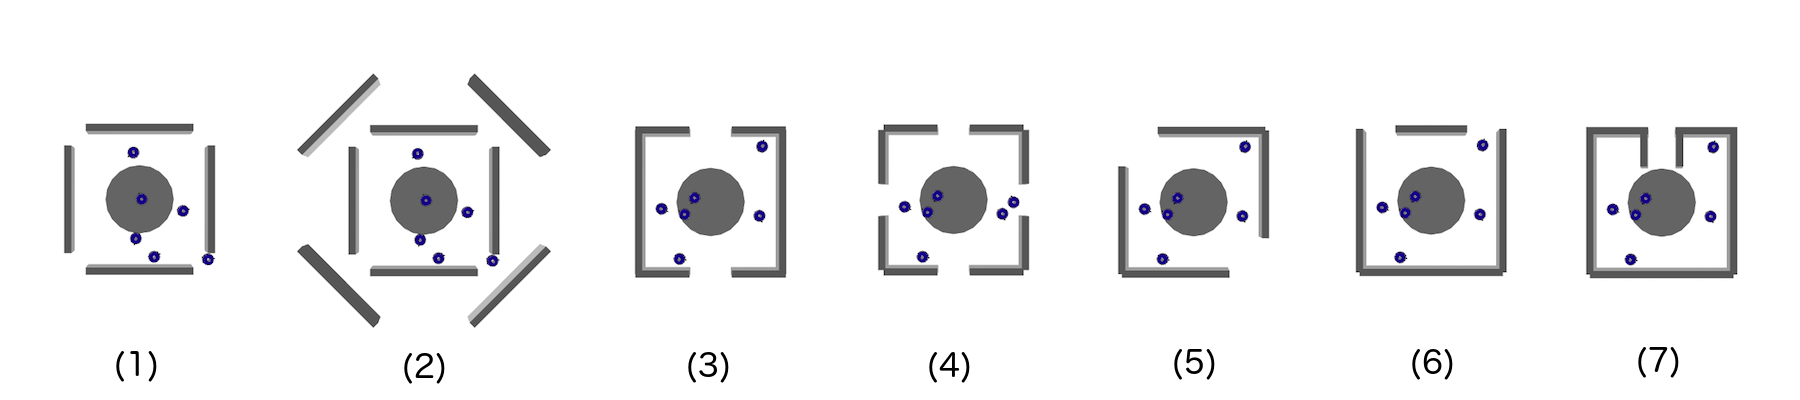
\includegraphics[width=18cm]{images/TrapTypes}
\caption{The set of traps used ordered in increasing estimated difficulty.} \label{fig:Traps}
\end{figure*}

\subsection{Double Bridge Experiment}

We attempted to replicate the double bridge experiment\cite{dorigo:aco}, using the ARGoS simulator. This required building an arena with one food cluster and two paths leading from the nest to the food. This proved difficult, and lead to an overall failure, as building paths in ARGoS was cumbersome. Built into the ARGoS simulator, ants are programmed to avoid the edge of the arena. This behavior worked well but was different than the ant behavior when an ant encountered an object, such as a wall forming a bridge to the food. This lead to ants getting stuck, attempting to navigate around walls. Furthermore, we were unable to reposition the nest to be decentralized, while still placing food around the arena. Food was always placed relative to the nest. 

The above complications lead to the double bridge arena shown in Figure \ref{fig:DoubleBridge}.

\begin{figure*}[ht]
\centering
\subfloat[][]{
\includegraphics[width=9cm]{images/DoubleBridgeEq}
 }
\subfloat[][]{
\includegraphics[width=9cm]{images/DoubleBridgeUnEq}
 }
\caption{(a) The double bridge arena in which each path is of equal length, from nest to food. (b) The double bridge arena in which one path is longer than the other, from nest to food.} \label{fig:DoubleBridge}
\end{figure*}

Despite difficulties, ants were able to leave the nest and collect food. However, they always followed the same pattern: leave the nest on the left of the arena, travel along the top path, pick up food, and bring it back to the nest along the bottom path. No ants ever went in the opposite direction, and the majority of the ants were stuck in the nest. This pattern held true for both double bridge arenas.

The failure of this experiment to correctly replicate Dorigo's\cite{dorigo:aco} experiment is primarily due to our inability to recreate an appropriate test environment. More tools for arena building are needed to properly recreate this experiment.

\keywords{
\textbf{GA: Genetic Algorithm} - An algorithm which generates each individual from some encoded form known as a "chromosome" or "genome". Chromosomes are combined or mutated to breed new individuals. "Crossover", the kind of recombination of chromosomes found in sexual reproduction in nature, is often also used in GAs. Here, an offspring's chromosome is created by joining segments chosen alternately from each of two parents' chromosomes which are of fixed length. GAs are useful for multidimensional optimization problems in which the chromosome can encode the values for the different variables being optimized.\cite{Dictionary.com2015} \\

\textbf{CPFA:} Central-Place Foraging Algorithm\cite{iAntArgosWiki}
\begin{itemize}
	\item \textbf{PSS:} Probability Of Switching To Searching
	\item \textbf{PRN:} Probability Of Returning To Nest
	\item \textbf{USV:} Uninformed Search Variation
	\item \textbf{RISD:} Rate Of Informed Search Decay
	\item \textbf{RSF:} Rate Of Site Fidelity
	\item \textbf{RLP:} Rate Of Laying Pheromone
	\item \textbf{RPD:} Rate Of Pheromone Decay
\end{itemize}
}

\textbf{OP:} Orientation-Position Vector
\begin{itemize}
	\item \textbf{ORIX:} Orientation X Value - The X value of the orientation vector.
	\item \textbf{ORIY:} Orientation Y Value (Fixed) - The Y value of the orientation vector.
	\item \textbf{ORIZ:} Orientation Z Value (Fixed) - The Z value of the orientation vector.
	\item \textbf{POSX:} Position X Value - The X value of the position vector.
	\item \textbf{POSY:} Position Y Value - The Y value of the position vector.
	\item \textbf{POSZ:} Position Z Value (Fixed) - The Z value of the position vector.
\end{itemize}
}

\section{Discussion}

One of the most challenging aspects of this project was learning how interpret data from such a vast search space with so many interconnected variables. However, we were able to successfully create GA that developed strategies for a variety of environments. By bounding variables to reasonable values, we were able to limit the search space, while allowing the GA explore many possible solutions. This process uncovered some interesting patterns shared amongst all of our environments.

Even with the impedance of traps, the GA produced fit swarms which performed comparably to environments without traps. The swarms were often able to use their collision avoidance techniques to easily navigate around traps. Only in the most difficult traps were they significantly hindered.

A pattern that emerged was how much time the GA required to discover an optimal solution, for a given environment, scaled proportionally to the difficulty of the trap. More difficult traps such as (6) and (7) require stricter bounds on certain parameters to be effective at all since even a small change in these parameter can lead to swarms being ineffective.

\section{Methods}
This section details the methods used to conduct the experiments.

\subsection{Genetic Algorithm}

\begin{table}[h]
\begin{tabular}{@{}ll@{}}
\toprule
Parameter              & Value      \\ \midrule
Population Size        & 40         \\
Elite Size             & 8          \\
Generations            & 40         \\
Mutational Probability & 10\%       \\
Simulation Duration    & 30 Minutes \\
Number of Food Tags    & 256        \\ 
Number of Ants         & 6          \\ 
Number of Obstacles    & 4          \bottomrule
\end{tabular}
\caption{Shows the exact parameters used for the GA.}
\label{table:gaParams}
\end{table}

The GA begins by initializing a population of iAnts swarms and obstacles. Initialization consists of forming a set of CPFA parameters for each iAnt swarm and a set of OP vectors for each obstacle. Both of these parameter sets are uniformly distributed over [0, 1] (scaled) with a offsets determined by sampling a normal distribution.

Lower and upper bounds are imposed on both the CPFA parameters and OP vectors to reduce the search space and exclude what are deemed as infeasible solutions. Such bounds are determined on a case-by-case basis; usually discovered by trial and error.

\begin{table}[h]
\begin{tabular}{@{}lll@{}}
\toprule
Parameter & Lower Bound & Upper Bound \\ \midrule
PSS       & 0.0         & 1.0         \\
PRN       & 0.0         & 1.0         \\
USV       & 0.0         & 180.0       \\
RISD      & 0.0         & 1.0         \\
RSF       & 0.0         & 20.0        \\
RLP       & 0.0         & 20.0        \\
RPD       & 0.0         & 1.0         \\ \bottomrule
\end{tabular}
\caption{The upper and lower bounds imposed on CPFA parameters.} \label{table:cpfaBounds}
\end{table}

\begin{table}[h]
\begin{tabular}{@{}lll@{}}
\toprule
Parameter    & Lower Bound & Upper Bound \\ \midrule
ORIX         & 0.0         & 90.0        \\
ORIY (Fixed) & 0.0         & 0.0         \\
ORIZ (Fixed) & 0.0         & 0.0         \\
POSX         & 1.5         & 5.0         \\
POSY         & 1.5         & 5.0         \\
POSZ (Fixed) & 0.0         & 0.0         \\ \bottomrule
\end{tabular}
\caption{The upper and lower bounds imposed on OP vectors.} \label{table:opBounds}
\end{table}

A random seed is generated for each simulation, then simulations are run and the fitness of each swarm is determined. At the end of each generation, elite individuals in the 80th percentile are chosen based on fitness. Remaining individuals are reformed by means of uniform crossover between randomly chosen individuals in the elite population followed by mutation. Each CPFA parameter has a 10\% chance to undergo mutation. Mutation is determined by taking a sample from a normal distribution with a mean equal to the current value of the parameter and a scaled standard deviation of 0.05. We have found that scaling the standard deviation relative to CPFA bounds prevents premature convergence to suboptimal solutions. The GA is run on each type of food distribution. We have found that optimal solutions are achieved after to \_ generations depending on the type of food distribution.

\subsection{Analysis Method}

Python's "subprocess" module provided us with the capability of readily switching between our program code and the simulation code. Simulations are performed in a large-scale autonomous robot simulator - ARGoS. Additionally, extensive usage of the Python modules "numpy" and "plot.ly" allowed us to perform data collection, analysis, and visualization with ease. All other segments of the program such as the GA were also written in Python.


% The following two commands are all you need in the
% initial runs of your .tex file to
% produce the bibliography for the citations in your paper.
\bibliographystyle{abbrv}
\bibliography{JJN-TMS-Project3}
%\balancecolumns
\appendix
\section{Plot.ly Page}\label{sec:one}
Plots shown in this paper can be viewed at https://plot.ly/$\sim$Zivia\section{Bitbucket Page}\label{sec:two}
The code repository can be found at https://bitbucket.org/Zivia/cs423/ This is a private repository and to gain access to this page you must be added as a contributor. Contact the author to be added.

\end{document}